\chapter{Uso do simulador}
\label{chap:uso_simulador}

\lettrine{N}{este} capítulo explícase brevemente como empregar o simulador, explicando cómo xerar os arquivos .elf e empregar o simulador, así como interpretar os resultados. 

O primeiro paso é empregar Segger Embedded Studio for RISC-V, aquí escribirase o código C para o programa que executará o simulador. Antes de compilar, tendo seleccionado no panel esquerdo Project [Nome do proxecto], débese modificar en Project -> Compiler como se mostra na \ref{fig:cap1}, é necesario elixir a extensión correcta. Por exemplo, no caso de que se realicen multiplicacións, débese cambiar de RV32I (por defecto) a RV32IM (ver \ref{fig:cap2}).

\begin{figure}[hp!]
  \centering
  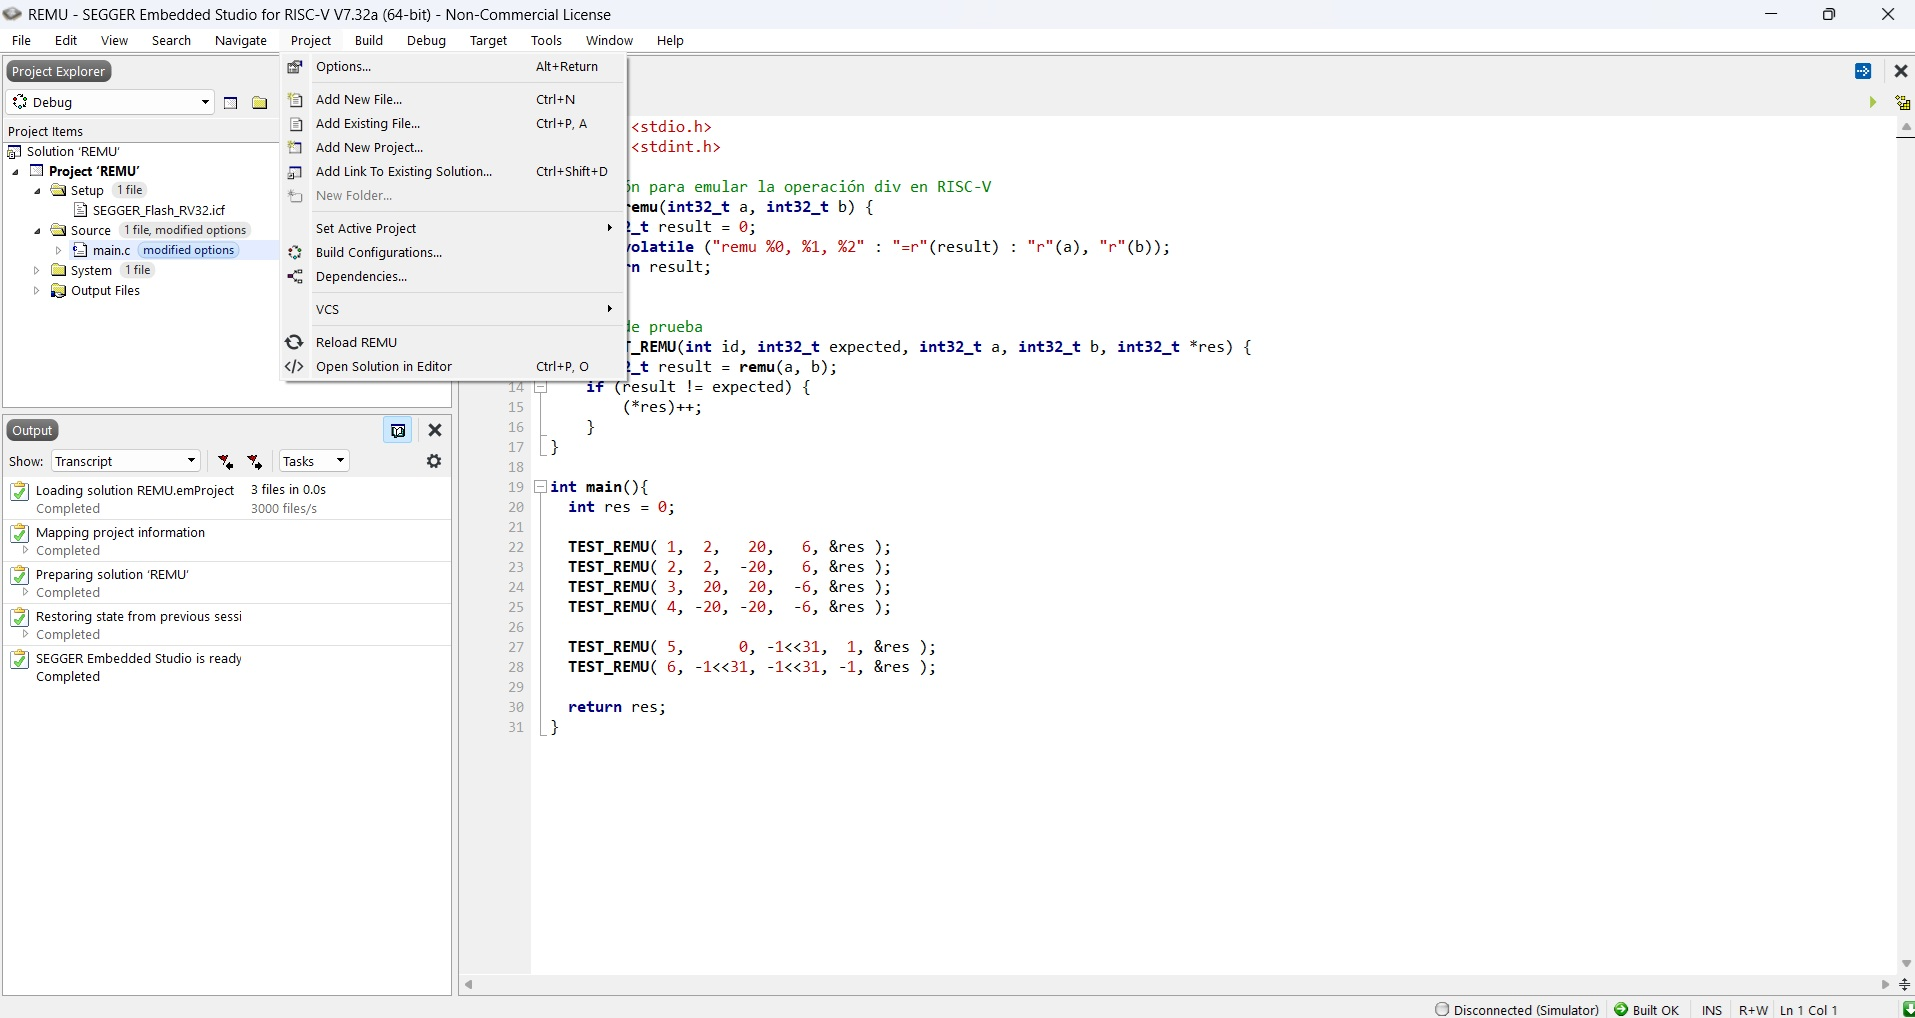
\includegraphics[width=\textwidth]{imaxes/Cap_1.jpg}
  \caption{Opcións do proxecto}
  \label{fig:cap1}
\end{figure}

\begin{figure}[hp!]
  \centering
  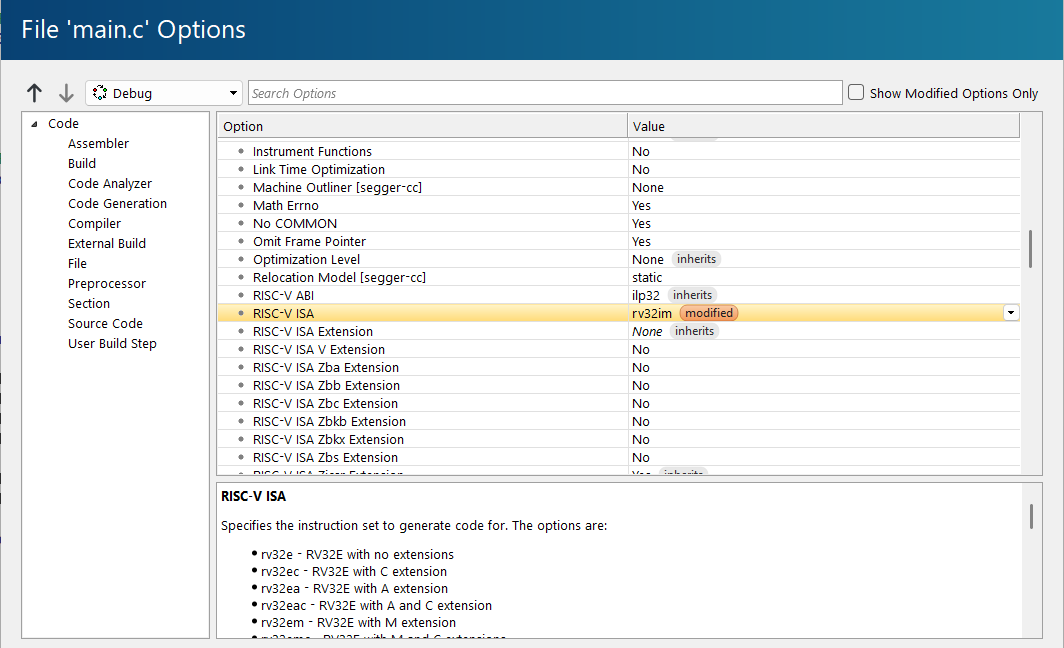
\includegraphics[width=\textwidth]{imaxes/Cap_2.png}
  \caption{Elección da extensión correcta}
  \label{fig:cap2}
\end{figure}

 Unha vez feito isto,  Build -> Build Solution, como mostra a captura \ref{fig:compilar}. Agora na carpeta Output Files, están varios arquivos, entre eles o executable con extensión .elf. É posible executar e depurar o código dentro do propio Segger, podendo así comprobar se o test está correcto de forma rápida (ver \ref{fig:cap3}).

\begin{figure}[hp!]
  \centering
  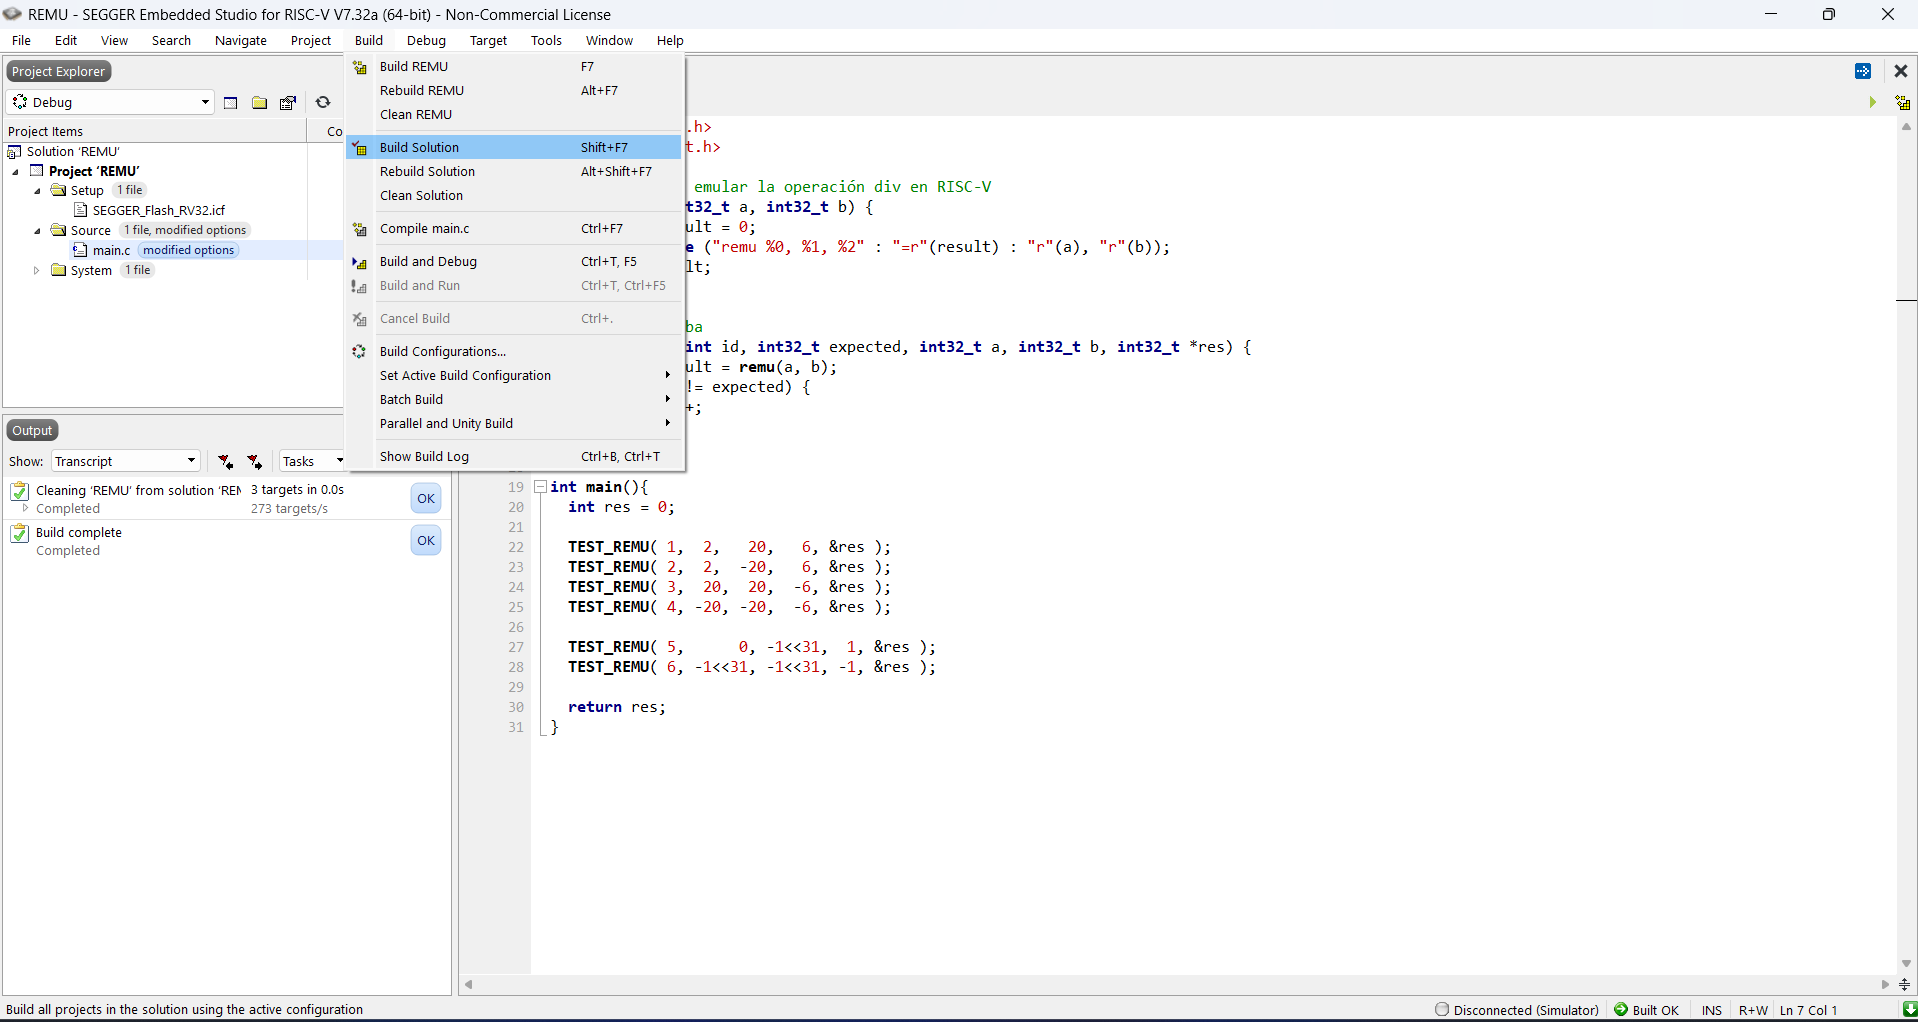
\includegraphics[width=\textwidth]{imaxes/Cap_3_Comp.png}
  \caption{Compilación do proxecto}
  \label{fig:compilar}
\end{figure}

\begin{figure}[hp!]
  \centering
  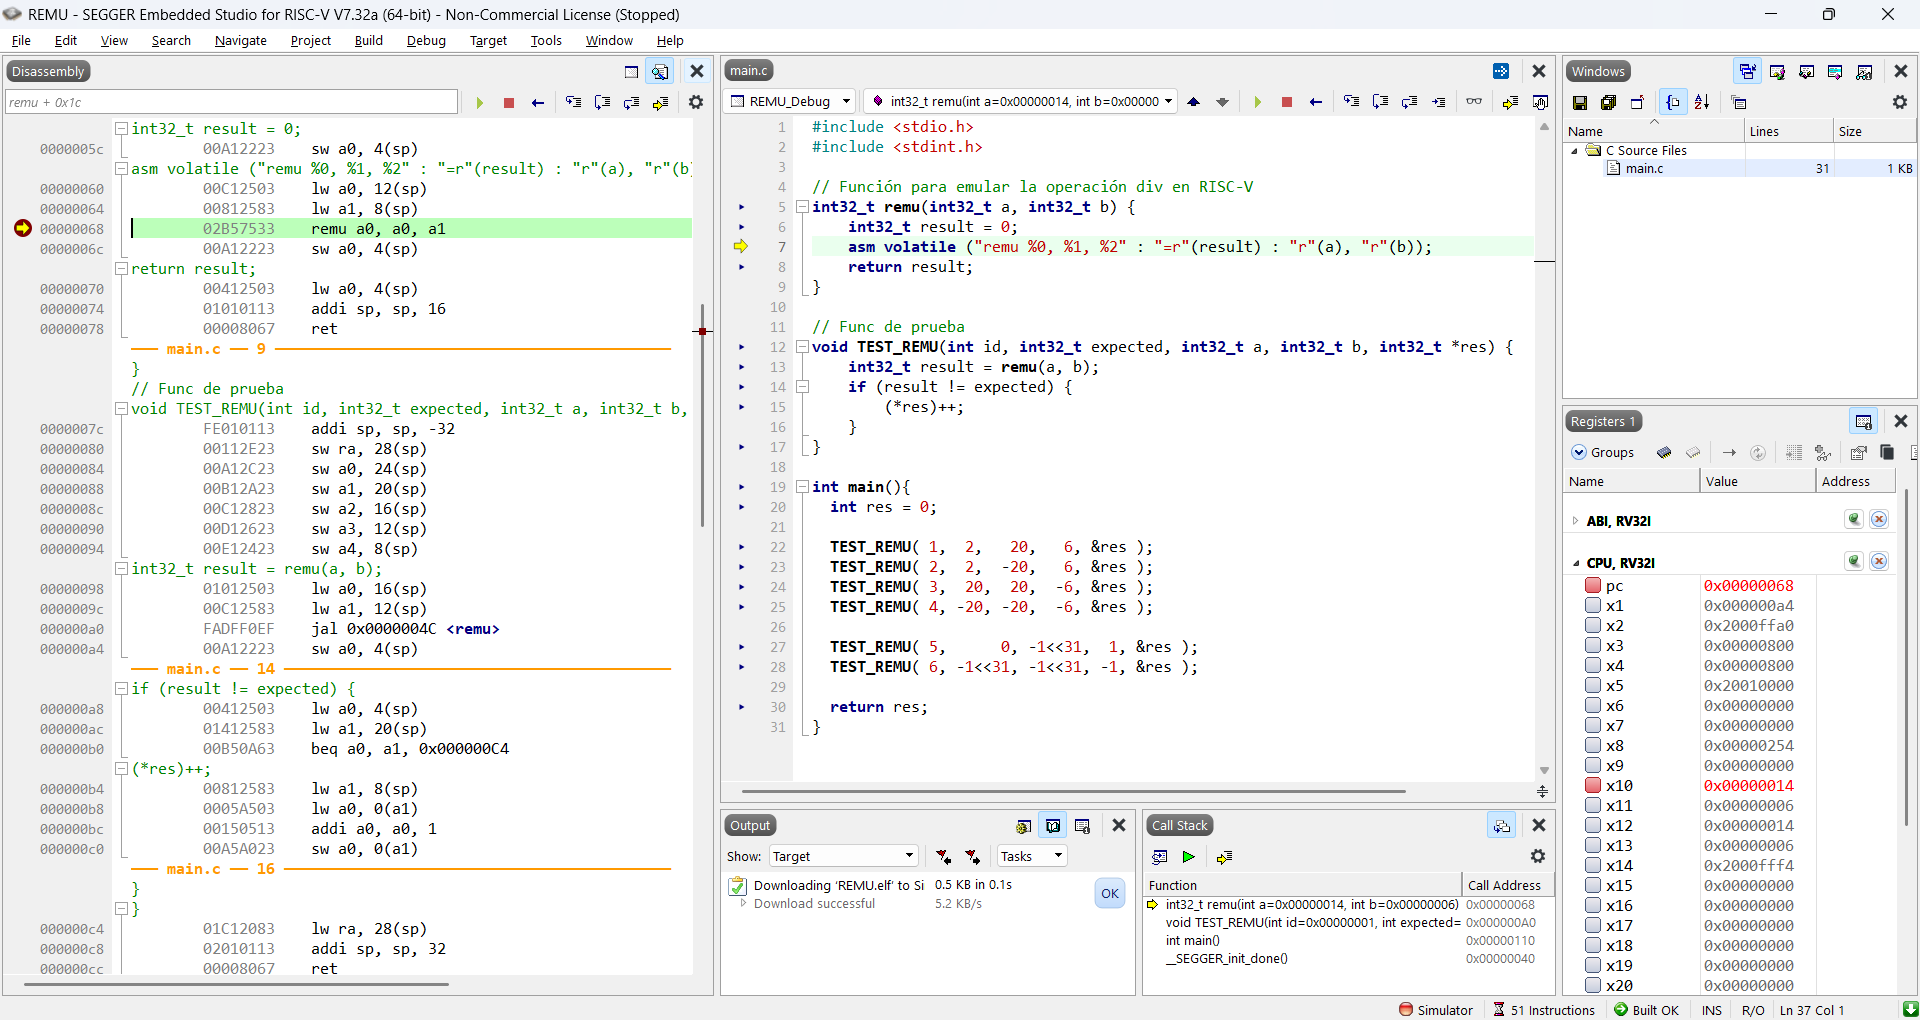
\includegraphics[width=\textwidth]{imaxes/Cap_4_Debug.png}
  \caption{Captura coas opcións de depuración de Segger}
  \label{fig:cap3}
\end{figure}

Para o axuste de parámetros debemos ir á Visual Studio 2022, no ficheiro config.h, aparecen definidas constantes para a latencia de instrucións, co nomes que seguen o formato LatencyNomeInstrución, por exemplo LatencyMul, como se ve na captura \ref{fig:parametros}. Finalmente, abrirase unha pantalla onde se mostrará que módulos están compilados, o tempo, o número de ciclos e o número de instrucións que levou o test. É importante revisar se o resultado é correcto, para isto, tal e como se mostra na \ref{fig:resultados} imprímese o valor do rexistro x10, onde se almacena un 0 se o resultado é o esperado ou 1 se hai algún erro.

\begin{figure}[hp!]
  \centering
  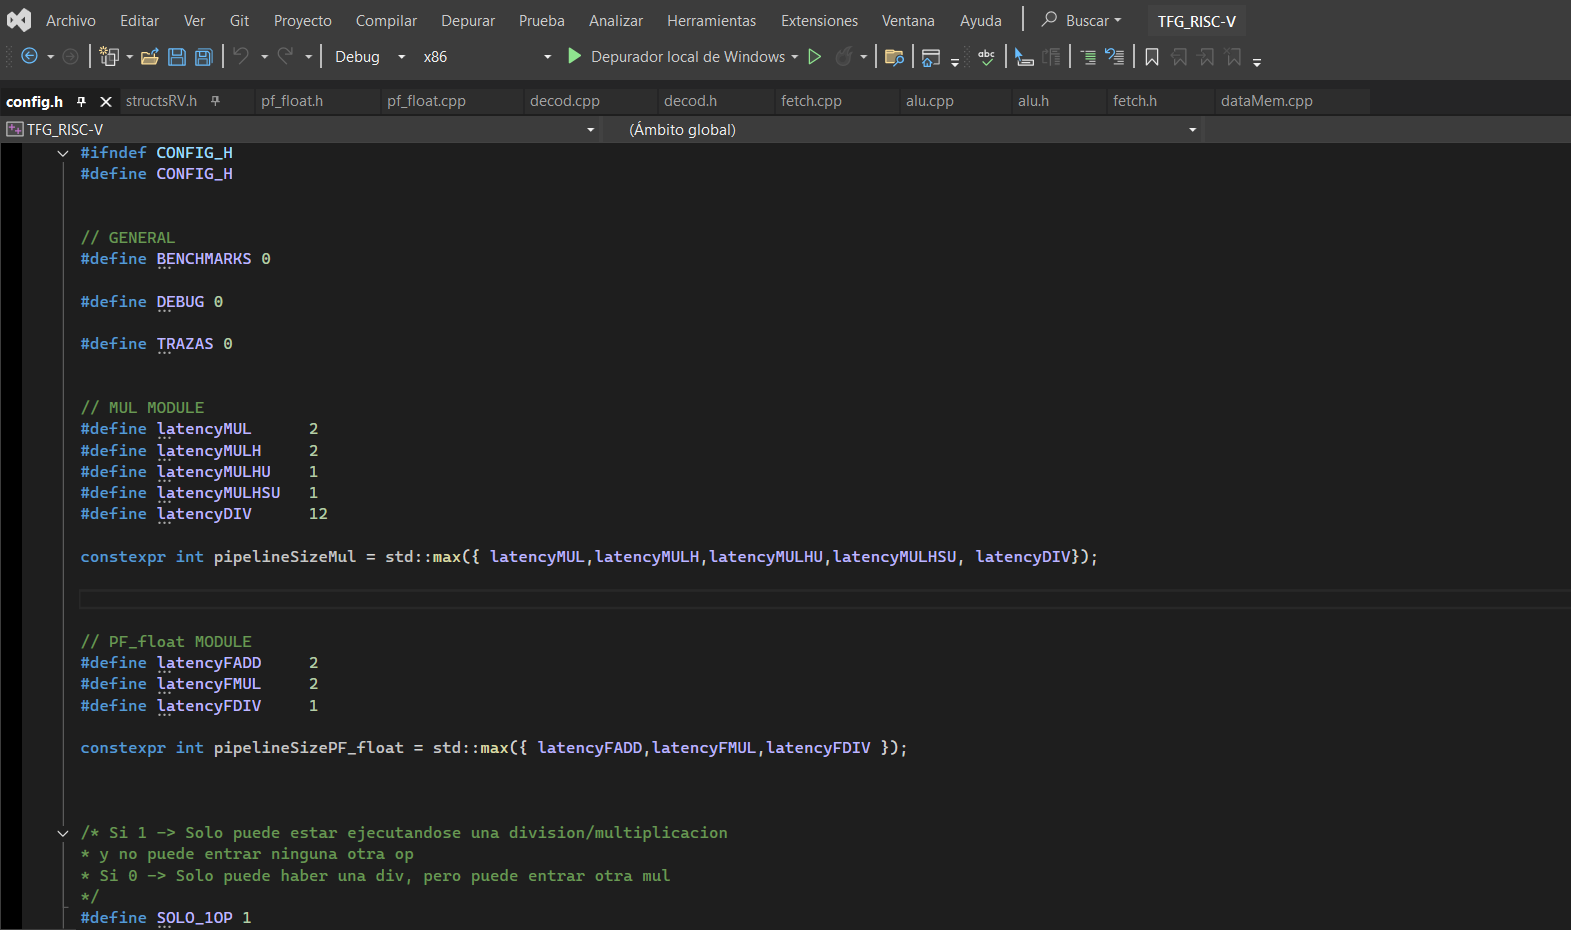
\includegraphics[width=\textwidth]{imaxes/Cap_5_Config.png}
  \caption{Cambio de parámetros en Config.h}
  \label{fig:parametros}
\end{figure}

\begin{figure}[hp!]
  \centering
  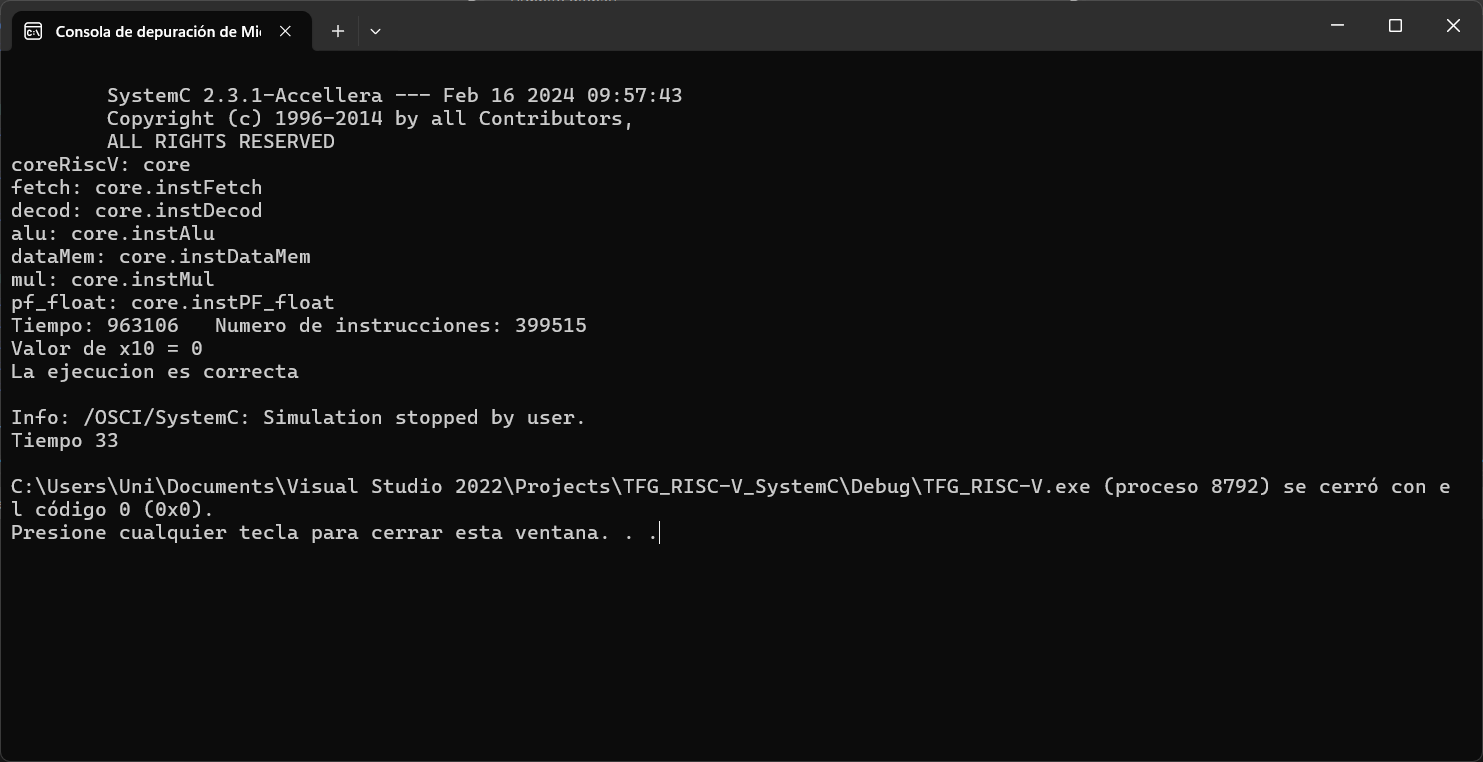
\includegraphics[width=\textwidth]{imaxes/Cap_res_final.png}
  \caption{Resultados tras executar o benchmark SPMV}
  \label{fig:resultados}
\end{figure}


